\documentclass{article}

\usepackage{graphicx}
\usepackage{tikz}
\usepackage{tikzsymbols}
\usetikzlibrary{calc,patterns,shapes.geometric}
\pagestyle{empty}
\usepackage[margin=0pt]{geometry}
\geometry{papersize={14in,12in}}

\def\centerarc[#1](#2)(#3:#4:#5){\draw[#1] ($(#2)+({#5*cos(#3)},{#5*sin(#3)})$) arc (#3:#4:#5);}

\begin{document}
	\begin{figure}
		\centering
		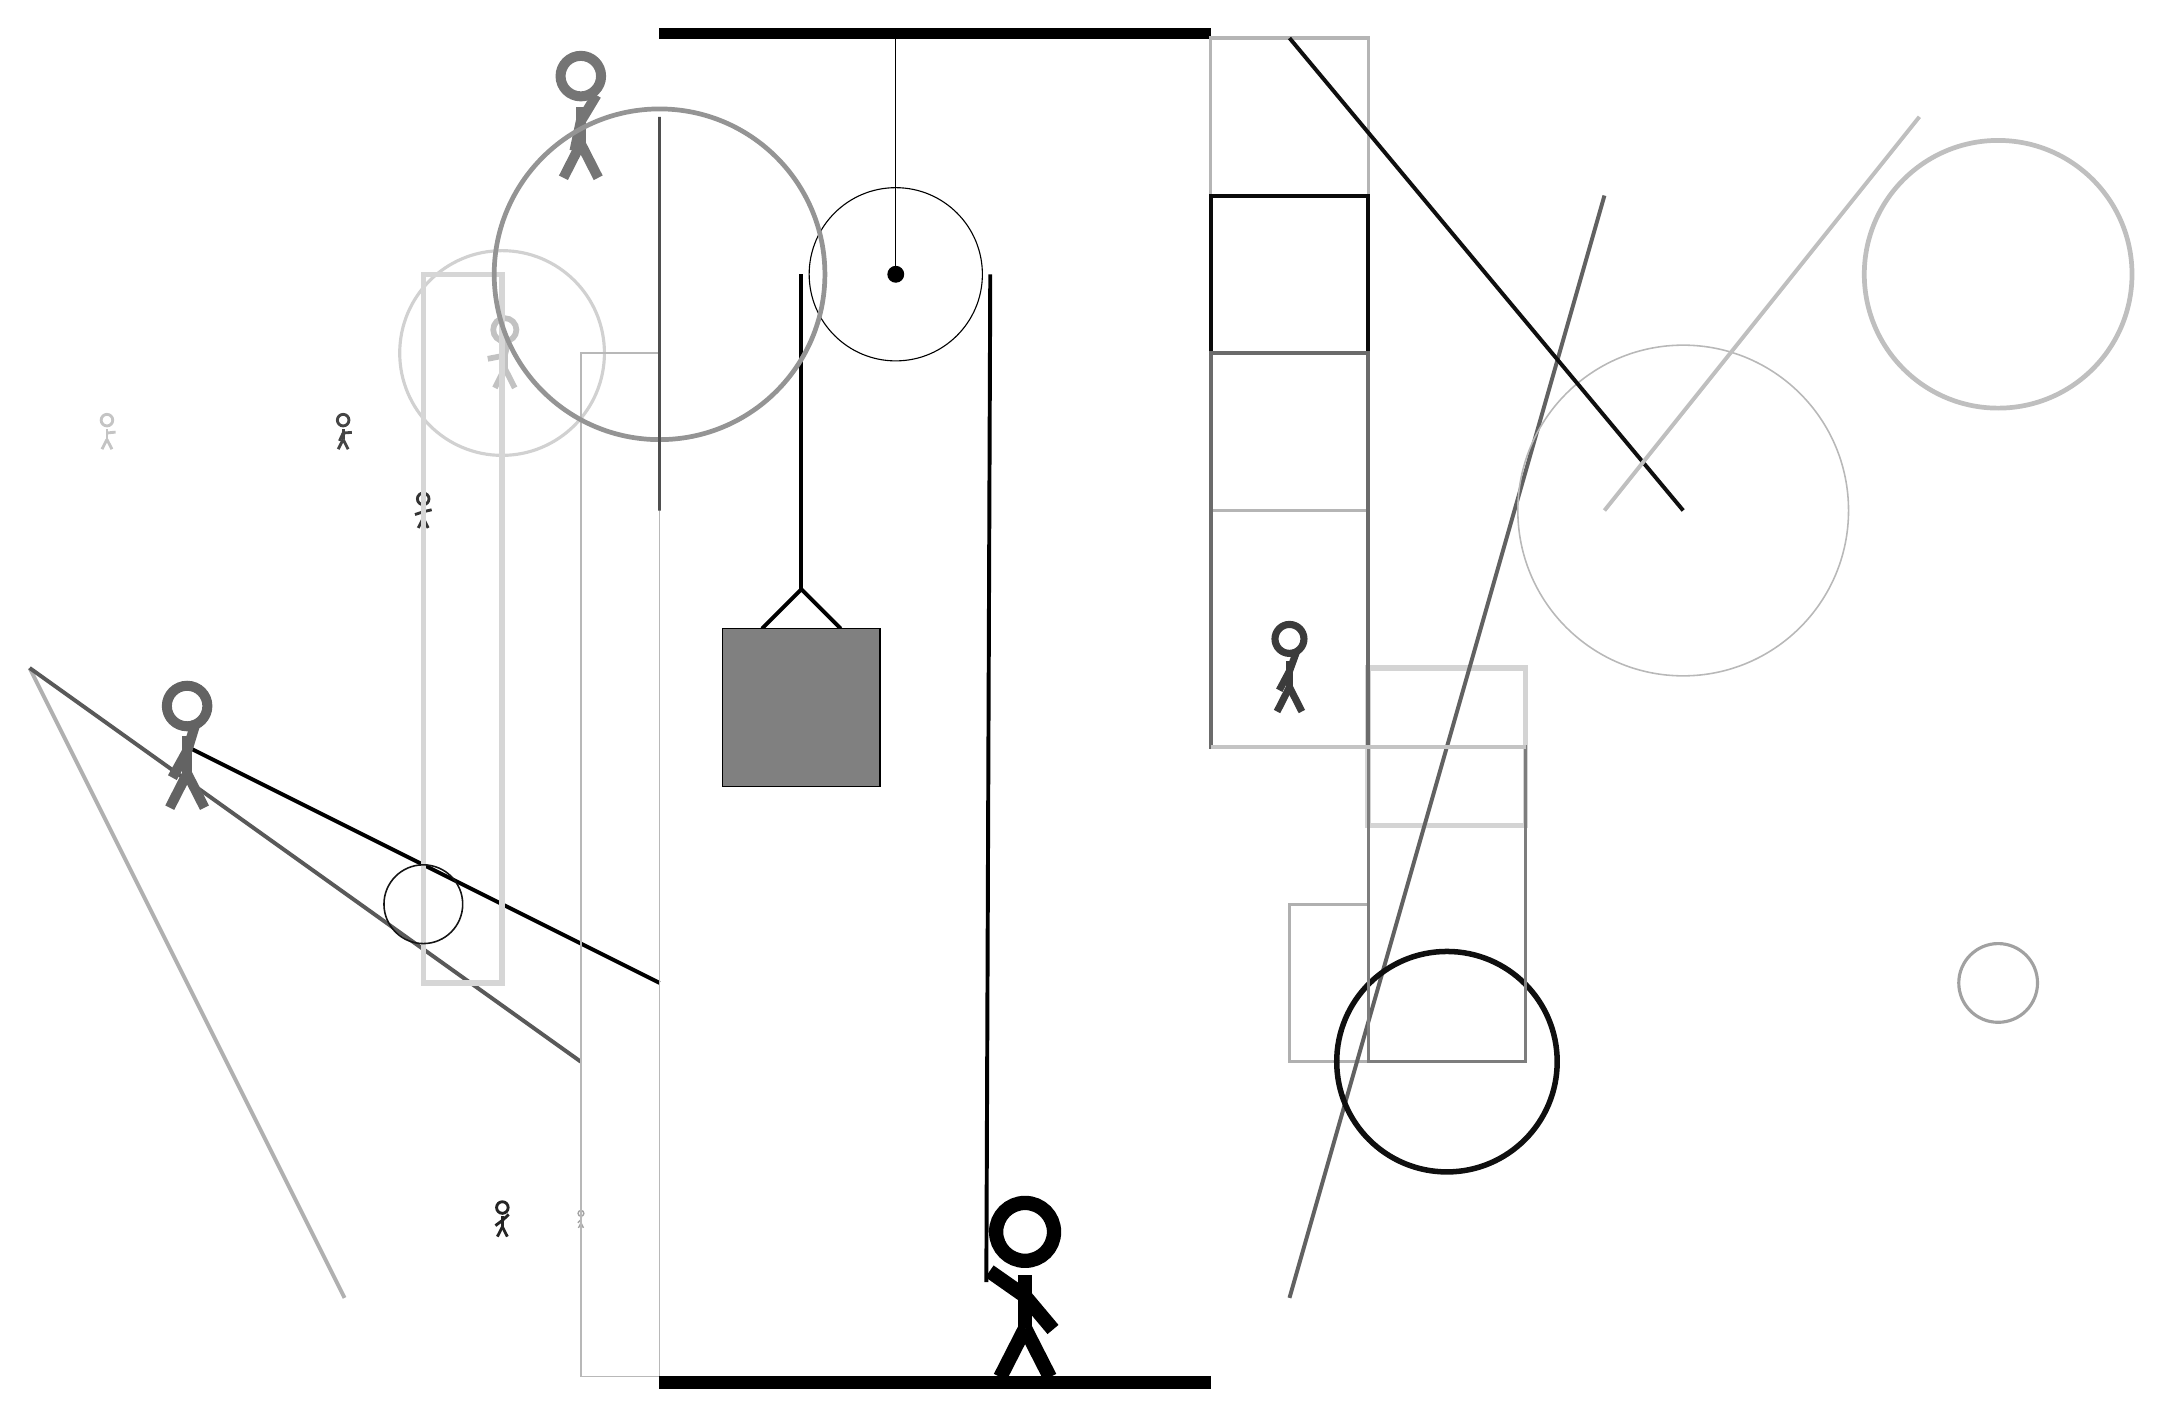
\begin{tikzpicture}
			%%%%% START %%%%%
			
			\draw[fill=black] (-2, 14) rectangle (5, 14.125);
			
			\draw (1, 11) circle (1.1);
			\draw[fill=black] (1, 11) circle (0.1);
			\draw (1, 14) -- (1, 11);
			
			\draw[line width=0.5mm] (-0.7, 6.5) -- (-0.2, 7.0) -- (0.3, 6.5);
			\draw[fill=black!50] (-1.2, 6.5) rectangle (0.8, 4.5);
			
			\draw[line width=0.5mm] (-0.2, 11) -- (-0.2, 7.0);
			\centerarc[line width=0.5mm](1, 11)(0:180:1.2000000000000002);
			\draw[line width=0.5mm](2.2, 11) -- (2.15, -1.8);
			
			\draw[line width=0.5mm, color=black!100](-2, 2) -- (-8, 5);
			
			\node[line width=0.2mm, color=black!73] at (-6, 9) {\Strichmaxerl[2][65][4]};
			\draw[line width=0.7mm, color=black!17] (7, 6) rectangle (9, 4);
			\node[line width=0.3mm, color=black!36] at (-3, -1) {\Strichmaxerl[1][43][82]};
			\draw[line width=0.5mm, color=black!31](-6, -2) -- (-10, 6);
			\node[line width=0.2mm, color=black!86] at (-4, -1) {\Strichmaxerl[2][37][43]};
			
			\draw[line width=0.4mm, color=black!31] (6, 3) rectangle (7, 1);
			\draw[line width=0.4mm, color=black!29] (7, 8) rectangle (5, 14);
			\node[line width=0.5mm, color=black!24] at (-4, 10) {\Strichmaxerl[4][11][76]};
			\node[line width=0.4mm, color=black!80] at (-5, 8) {\Strichmaxerl[2][19][13]};
			\node[line width=0.2mm, color=black!54] at (-3, 13) {\Strichmaxerl[7][78][59]};
			
			\draw[line width=0.5mm, color=black!62](6, -2) -- (10, 12);
			\node[line width=0.4mm, color=black!77] at (6, 6) {\Strichmaxerl[5][62][70]};
			\draw[line width=0.5mm, color=black!65](-3, 1) -- (-10, 6);
			\draw [line width=0.6mm, color=black!25](15, 11) circle (1.7);
			\draw [line width=0.2mm, color=black!28](11, 8) circle (2.1);
			
			\draw[line width=0.3mm, color=black!13] (7, 3) rectangle (7, 6);
			\draw [line width=0.4mm, color=black!18](-4, 10) circle (1.3);
			\draw[line width=0.2mm, color=black!28] (-2, -3) rectangle (-3, 10);
			
			\draw[line width=0.5mm, color=black!94](6, 14) -- (11, 8);
			\draw [line width=0.7mm, color=black!94](8, 1) circle (1.4);
			
			\node[line width=0.4mm, color=black!23] at (-9, 9) {\Strichmaxerl[2][90][6]};
			
			\draw[line width=0.5mm, color=black!96] (7, 10) rectangle (5, 12);
			\draw[line width=0.7mm, color=black!16] (-4, 11) rectangle (-5, 2);
			\node[line width=0.4mm, color=black!61] at (-8, 5) {\Strichmaxerl[7][61][73]};
			
			\draw [line width=0.6mm, color=black!42](-2, 11) circle (2.1);
			
			\draw[line width=0.5mm, color=black!58] (7, 10) rectangle (5, 5);
			\draw [line width=0.4mm, color=black!37](15, 2) circle (0.5);
			
			\draw[line width=0.5mm, color=black!25](10, 8) -- (14, 13);
			\draw[line width=0.4mm, color=black!51] (7, 1) rectangle (9, 5);
			\draw[line width=0.3mm, color=black!69] (-2, 13) rectangle (-2, 8);
			
			\draw [line width=0.2mm, color=black!92](-5, 3) circle (0.5);
			\draw[line width=0.5mm, color=black!23](5, 5) -- (9, 5);
			
			\node at (2.6, -1.9) {\Strichmaxerl[10][-35][-50]};
			
			\draw[fill=black] (-2, -3) rectangle (5, -3.15);
			
			%%%%% END %%%%%
		\end{tikzpicture}
	\end{figure}	
\end{document}